% ---- ETD Document Class and Useful Packages ---- %
\documentclass{ucetd}
\usepackage{subfigure,epsfig,amsfonts}
\usepackage{natbib}
\usepackage{amsmath}
\usepackage{amssymb}
\usepackage{amsthm}
\usepackage[toc,page]{appendix}
\usepackage[labelfont=bf]{caption}
\usepackage{rotating}
\usepackage[dvipsnames]{xcolor}
\usepackage{url}
\usepackage{bm}
\usepackage{bbm}

%% Use these commands to set biographic information for the title page:
\title{Visualizing nucleosome cluster dynamics with stochastic optical reconstruction microscopy}
\author{Clayton W. Seitz}
\department{Department of Physics}
\division{Physical Sciences}
\degree{Doctor of Philosophy}
\date{Spring 20XX}

%% Use these commands to set a dedication and epigraph text

\epigraph{Epigraph}



\begin{document}
%% Basic setup commands
% If you don't want a title page comment out the next line and uncomment the line after it:
%\maketitle
%\omittitle

% These lines can be commented out to disable the copyright/dedication/epigraph pages
%\makecopyright
%\makededication


%% Make the various tables of contents
\tableofcontents
%\listoffigures
%\listoftables

%\acknowledgments
% Enter Acknowledgements here

\abstract

Single-molecule localization microscopy (SMLM) techniques, such as direct stochastic optical reconstruction microscopy (dSTORM), can be used to produce a pointillist representation of nucleosome organization at diffraction-unlimited precision. Direct STORM approaches leverage the deactivation of fluorescent tags, followed by spontaneous or photoinduced reactivation, which can be used to achieve super-resolution reconstructions of nuclear proteins and nucleic acids. This basic principle remains one of the method's primary limitations - standard SMLM fitting routines require tight control of activation and reactivation to maintain sparse emitters, presenting a tradeoff between imaging speed and labeling density. Here, we present a dSTORM strategy for fast reconstruction of nucleosome organization in living cells by complementing high duty-cycle blinking of rhodamine-derived dyes with a localization algorithm based on deep neural networks. By performing high density localization and two-color imaging, we intend to directly visualize nucleosome cluster dynamics and chromatin mobility following BRD4 inhibition with small molecule drugs JQ1 and 1,6 Hexanediol.


\clearpage

\mainmatter



\section{Introduction}

\subsection{Visualizing nucleosome cluster dynamics in BRD4 condensates at super-resolution}

The nucleosome is the fundamental structural unit of DNA packaging in eukaryotic cells. It consists of approximately 146 base pairs (bp) of DNA wrapped in 1.67 left-handed superhelical turns around a histone octamer, consisting of 2 copies each of the core histones H2A, H2B, H3, and H4. (Luger 1997). Super-resolved nucleosome organization has been studied extensively in various epigenomic states to reveal segregated nanoclusters, dispersed nanodomains, and compact large aggregates  8–10 . Nucleosomes assemble into heterogeneous clusters of variable sizes, interspersed with nucleosome-depleted regions (Ricci 2015). Histone modifications regulate the packaging of nucleosomes into a higher-order chromatin structure to influence the accessibility of genomic DNA to transcription machinery. Higher-order chromatin structure is implicated in a number of cellular processes including gene regulation (Hnisz 2017; Sabari 2018; Boija 2018), DNA damage and repair (Locatelli 2022), as well as cell differentiation and immune activation (Lin 2022).


Histones can be decorated with various post-translational modifications such as acetylation, methylation, phosphorylation, and ubiquination. The recruitment of proteins and complexes with specific enzymatic activities is now a well-accepted dogma of how modifications mediate their function. In this way, modifications can influence transcription of genes, and many other DNA processes such as repair, replication and recombination (Bannister and Kouzarides, 2011). Here, we study live-cell dynamics of nucleosome organization, with a particular focus on bromodomain protein 4 (BRD4) protein, a major tandem-bromodomain-containing transcriptional regulator. BRD4 plays an important role in diverse cellular functions such as transcription, replication, epigenetic regulation, and DNA repair, and has been implicated in cancer and autoimmune diseases. BRD4 acetylates H3 K122, a residue critical for nucleosome stability, resulting in nucleosome eviction and chromatin decompaction (Devaiah 2016). It functions as a scaffold for transcription factors at promoters and super-enhancers. Importantly, the intrinsically disordered regions (IDRs) of BRD4 are thought to facilitate its phase separation with coactivators such as MED1. Indeed, the IDRs of MED1 and BRD4 from phase separated liquid droplets in-vitro, which could be disrupted after addition of 1,6 Hexanediol (Sabari 2018).  

\subsection{Single molecule localization microscopy}

Single molecule localization microscopy (SMLM) relies on the temporal resolution of fluorophores in the sample whose spatially overlapping point spread functions would otherwise render them unresolvable at the detector. SMLM techniques, such as stochastic optical reconstruction microsscopy (STORM) and photoactivatable localization microscopy (PALM) remain desirable for super-resolution imaging of many cellular structures, due to their cost-effective implementation and photon-count limited resolution (Schermelleh 2019). Common strategies for the temporal separation of molecules involve transient intramolecular rearrangements to switch from dark to fluorescent states or the exploitation of non-emitting molecular radicals. For direct STORM, rhodamine derivatives can undergo intersystem crossing to a triplet state, which can reduced by thiols to form a dark radical species. The dark state can then be quenched by oxidative processes, driving the fluorophore back to its ground state (Figure 1). Long dark state lifetimes are commonly used in STORM imaging, while quenching results in higher duty cycle photoswitching and increased rates of photobleaching due to irreversible oxidative damage of important functional groups. Long dark state lifetimes are frequently achieved by using an oxygen scavenging buffer containing glucose oxidase, catalase, and others. 

Fluorescent labeling density has been known to pose a major bottleneck to super-resolution imaging acqusitions. Static uncertainty due to molecular crowding can be partially amelioriated by using pairwise or higher-order temporal correlations within a pixel neighborhood, known as stochastic optical fluctuation imaging (Dertinger 2009). Other approaches such as stimulated emission and depletion (STED) imaging bring control over the photophysical state of a chosen subset of the sample, yet the need for laser scanning prevents widespread application in live-cell studies. 

\begin{figure}
\begin{center}
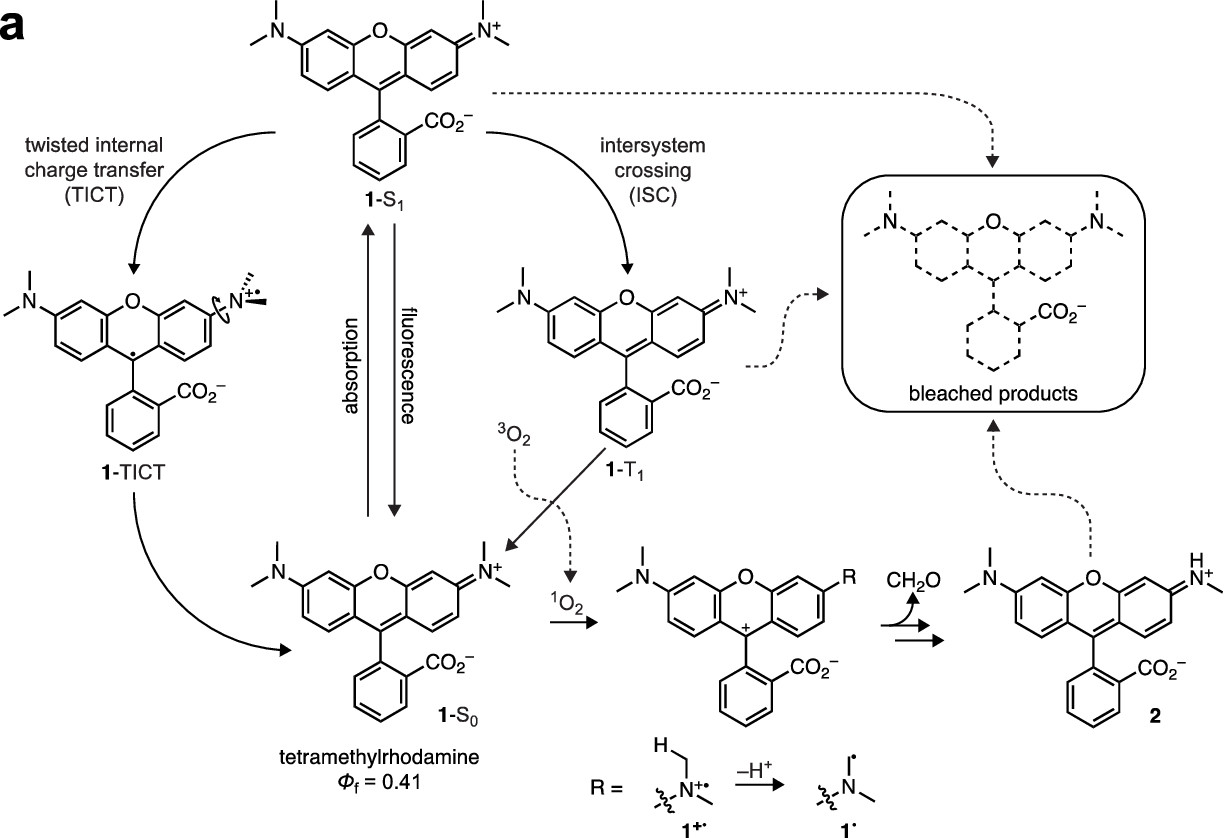
\includegraphics[width=14cm]{Rhodamines.png}
\end{center}
\caption{Photophysics of tetramethylrhodamine (TMR) and its derivatives Janelia-Fluor (JF)549 and JF646. Maximum absorption occurs at 549nm or 646nm respectively and return to the ground state can occur via twisted internal charge transfer or inter-system crossing.}
\end{figure}


Furthermore, the spatial resolution and relative simplicity of SMLM techniques remains unmatched, inciting an effort to increase the time resolution of STORM and PALM methods. Previous approaches to breaking the time resolution barrier in SMLM fall into two main categories: generative models and dense localization methods. Generative methods learn prior information about cellular structures from super-resolution images, which is used to predict super-resolution images based on sparse localizations or widefield images (Ouyang 2018; Barth 2020; Chen 2023). Other approaches use convolional neural networks to interpolate and transform dense images into a localization map (Nehme 2020; Speiser 2021). Here, we adapt the latter methodology, as biological structures such as chromatin are dynamic and intrinsically heterogeneous; therefore, structures cannot necessarily be known apriori, and deep generative models can hallucinate image artifacts. In any case, dense localization remains a hard problem and is highly application specific, and the following paragraphs will develop a method from first principles for precision super-resolution imaging of nucleosomes


\subsection{Estimator precision sets the resolution limit in localization microscopy}

In recent years, Complementary Metal-Oxide-Semiconductor (CMOS) cameras have become a central tool in fluorescence microscopy. The CMOS sensor is revered for its high frame rates, allowing researchers to reach higher temporal resolutions. Nevertheless, CMOS cameras have noise sources intrinsic to their operation, such as shot noise and readout noise. The former phenomenon can describe a superposition of processes; namely, the fluctuations of the number of photons due to the quantum nature of light, and the random conversion of photons into photoelectrons within the semiconductor material with a quantum efficiency below unity. Here we will often refer to the photon count $N_{0}$, which has a determined value, rather than being described by statistically. The \emph{measured} photon count, however, is well-described by a Poisson process (Schottky 1918). A shot-noise limited image with $N$ pixels is then described as a family of Poisson variables, with units of photoelectrons


\begin{equation}
\vec{S} = \left[\mathrm{Poisson}(\mu_{1}), \mathrm{Poisson}(\mu_{2}), ..., \mathrm{Poisson}(\mu_{N})\right]
\end{equation}

CMOS sensors also suffer from other noise sources, such as readout noise or dark current, resulting in a nonzero signal even in the absence of incident light. Dark current is due to statistical fluctuations in the photoelectron count within a semiconductor material in thermal equilibrium. Fortunately, these additional noise sources are governed by the central limit theorem, and can be efficiently summarized as the component of the noise which exhibits a Gaussian distribution. Readout noise has been often neglected in localization algorithms because its presence in EMCCD cameras is small enough that it can be ignored within the tolerances of the localization precision. In the case of high speed CMOS cameras, however, the readout noise of each pixel is significantly higher and, in addition, every pixel has its own noise and gain characteristic sometimes with dramatic pixel-to-pixel variations (Huang 2013). Therefore, accurate localization and simulation necessisitates models which incorporate detailed sensor properties. 


\section{Results}

\subsection{Dense two-dimensional and sparse three-dimensional SMLM}

Two major factors contribute to localization errors in SMLM: (i) the noise characteristics of CMOS cameras and (ii) crowding of molecules within a diffraction limited region. Maxmimum likelihood estimation is frequently used for isolated molecules and high signal levels, retaining localization errors from 30-40nm (Figure 3c). However, MLE performance tends to degrade in low SNR and dense regimes ($K(\lambda/2\mathrm{NA}) > 1$), requiring more sophisticated localization methods, such as convolutional neural networks (CNNs). CNNs have been widely adopted for imaging processing tasks in fluorescence microscopy (Weigert 2018; Ronneberger 2015). Here, we employ a localization CNN architecture based on DeepSTORM3D and consists of three main modules: the first consisting of successive dilated convolutions, followed by an upsampling module to increase the lateral resolution by a factor of 4. The third and last module adds additional convolutional blocks to refine localization estimates. This architecture can also be used for three-dimensional localization and thus the final output has $n_{z}$ channels. Of course, for two-dimensional localization $n_{z}=1$. The final output is followed by an element-wise HardTanh (Maas 2013). A post-processing function $F_{PP}$ uses a user-defined threshold to produce a matrix of coordinates. We find the performance of this architecture on simulated images surpasses MLE, and approaches the Cramer-Rao lower bound at high signal levels, retaining a RMSE near 20nm for $K(\lambda/2\mathrm{NA}) \leq 5$, at high signal levels (Figure 3c). 


To generalize our imaging setup to three-dimensions, we could use that the lateral point spread function has a weak dependence on the axial coordinate (Figure 3a). However, it has been shown that the error around the focus can be large, while negative and positive defocus cannot be distinguished given the symmetric dependence in $z$ (Holtzer 2007). Instead, we choose to introduce astigmatism into the detection path using a weak cylindrical lens (Figure 4a). In effect, this breaks the axial symmetry of the PSF and gives an anisotropic Gaussian which is elongated perpendicular to the optical axis. Localization proceeds by measuring this anisotropy and inverting a model of its axial dependence. At high numerical aperture, a strong dependence of the anisotropy to axial displacement potentially provides more precise three-dimensional localization (Figure 4b).  This axial anisotropy can be complex, but is often well described by a polynomial function of the axial displacement $z_{0}$ (Smith 2010). Unfortunately, astigmatic imaging increases the width of the point spread function significantly, exacerbating localization errors by molecular crowding and low signal to noise ratio. Therefore, we report error statistics for maximum likelihood based methods only, and leave three-dimensional localization with CNNs to future work. As one might expect, at ideal SNR, we show that axial dependence of localization error bears a strong similarity to the axial dependence of the PSF width (Figure 4c). Lateral RMSE can be maintained below 40nm for the anisotropic PSF for $K(\lambda/2\mathrm{NA}) \leq 5$; however, the Jaccard index tends to rapidly degrade at higher molecular densities, making MLE an unsuitable estimator for dense three-dimensional imaging (Figure 5). However, three-dimensional tracking with sparse emitters remains a good application of this method.

\begin{figure}
\begin{center}
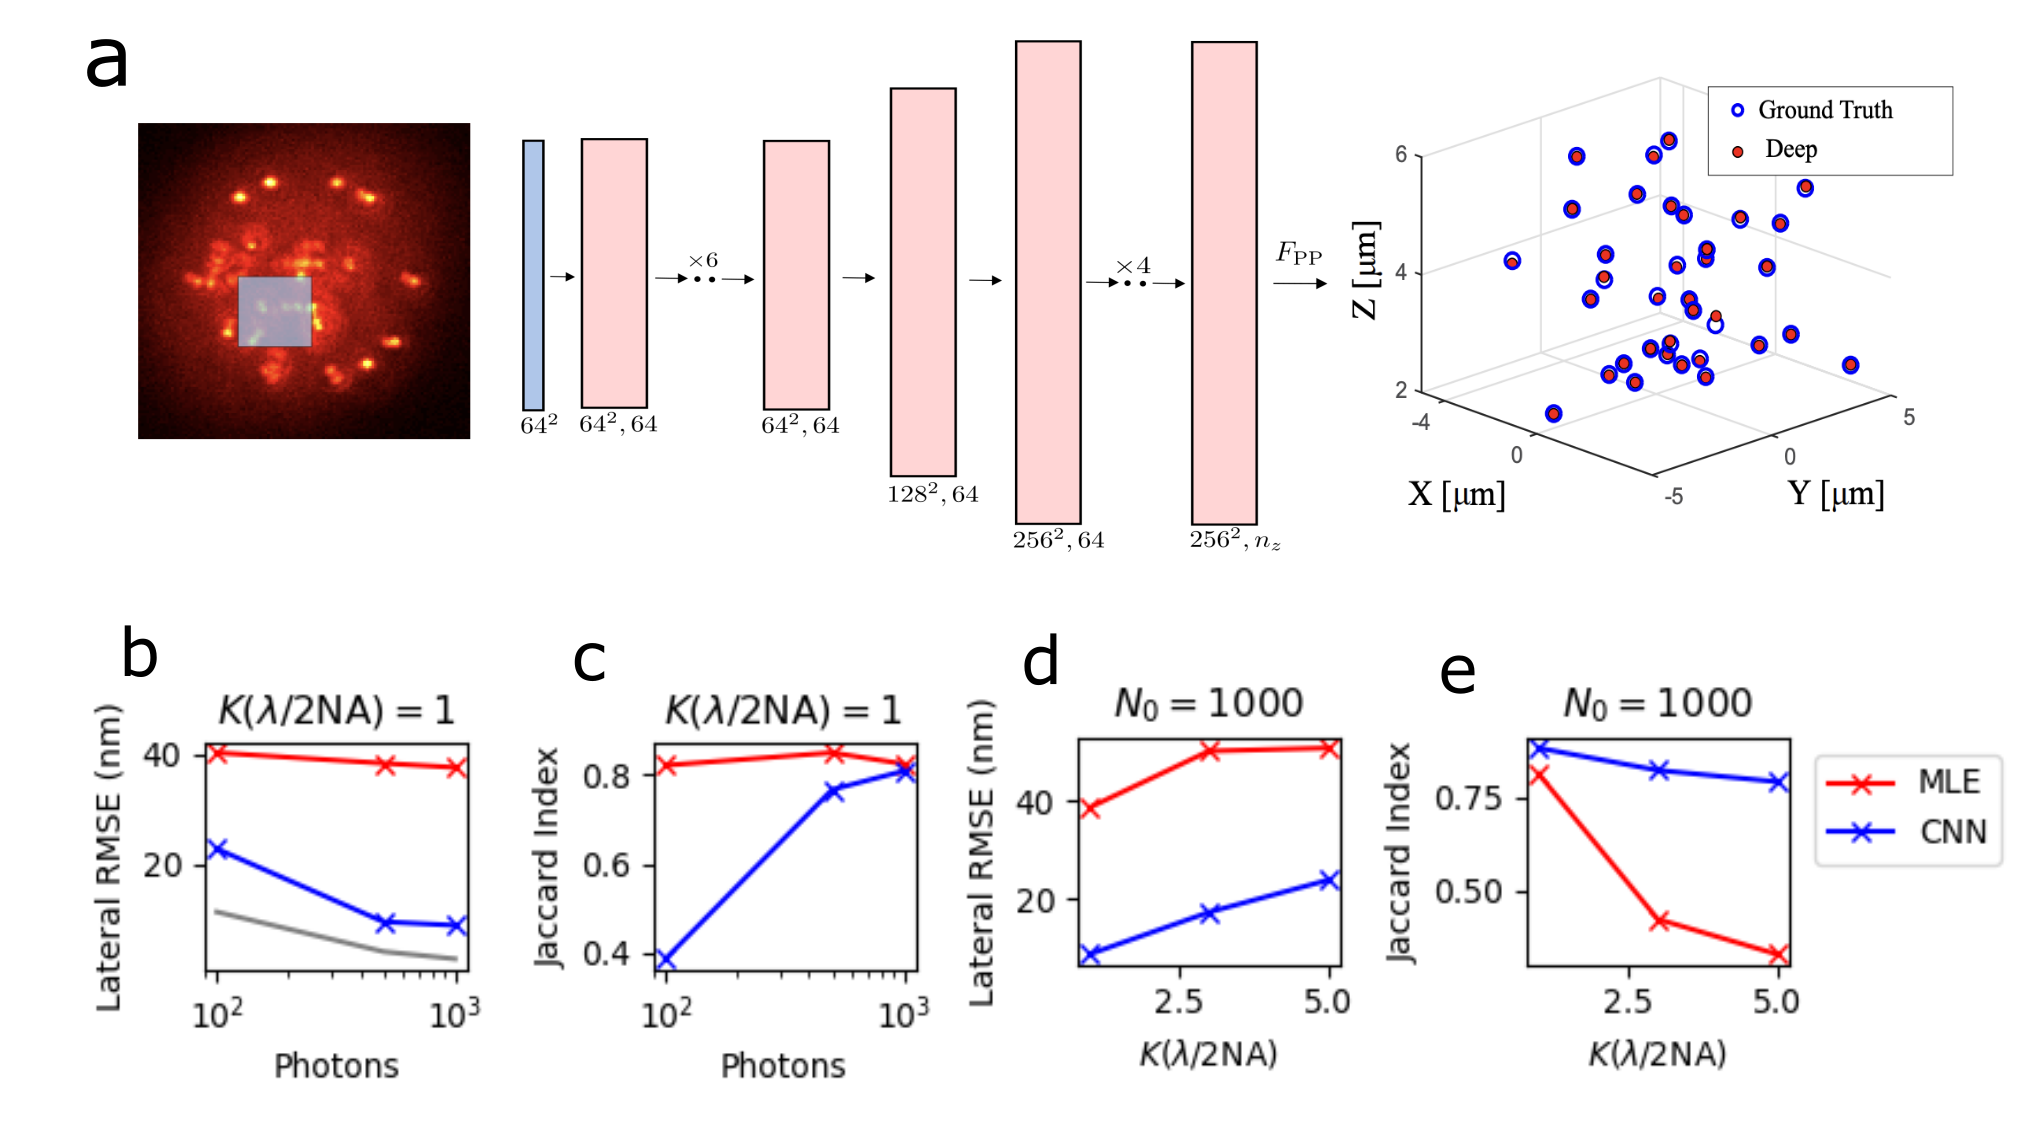
\includegraphics[width=14cm]{PSF2D.png}
\end{center}
\caption{Convolutional neural networks outperform MLE in dense and low-signal cases (A) Lateral and axial point spread functions for high ($\sim$1.25) and low ($\sim$0.8) numerical aperture (NA). (B) Convolutional neural network architecture used for localization. A monochrome image is convolved and upsampled to generate a localization map, which is post-processed to produce a vector of coordinates. (C) Lateral root mean squared error of maximum likelihood estimator (MLE) and a convolutional neural network (CNN) with respect to the incident photon count and the number of molecules within the diffraction limit $\lambda/2\mathrm{NA}$ for high NA. Error samples = $10^{3}$}
\end{figure}



\begin{figure}
\begin{center}
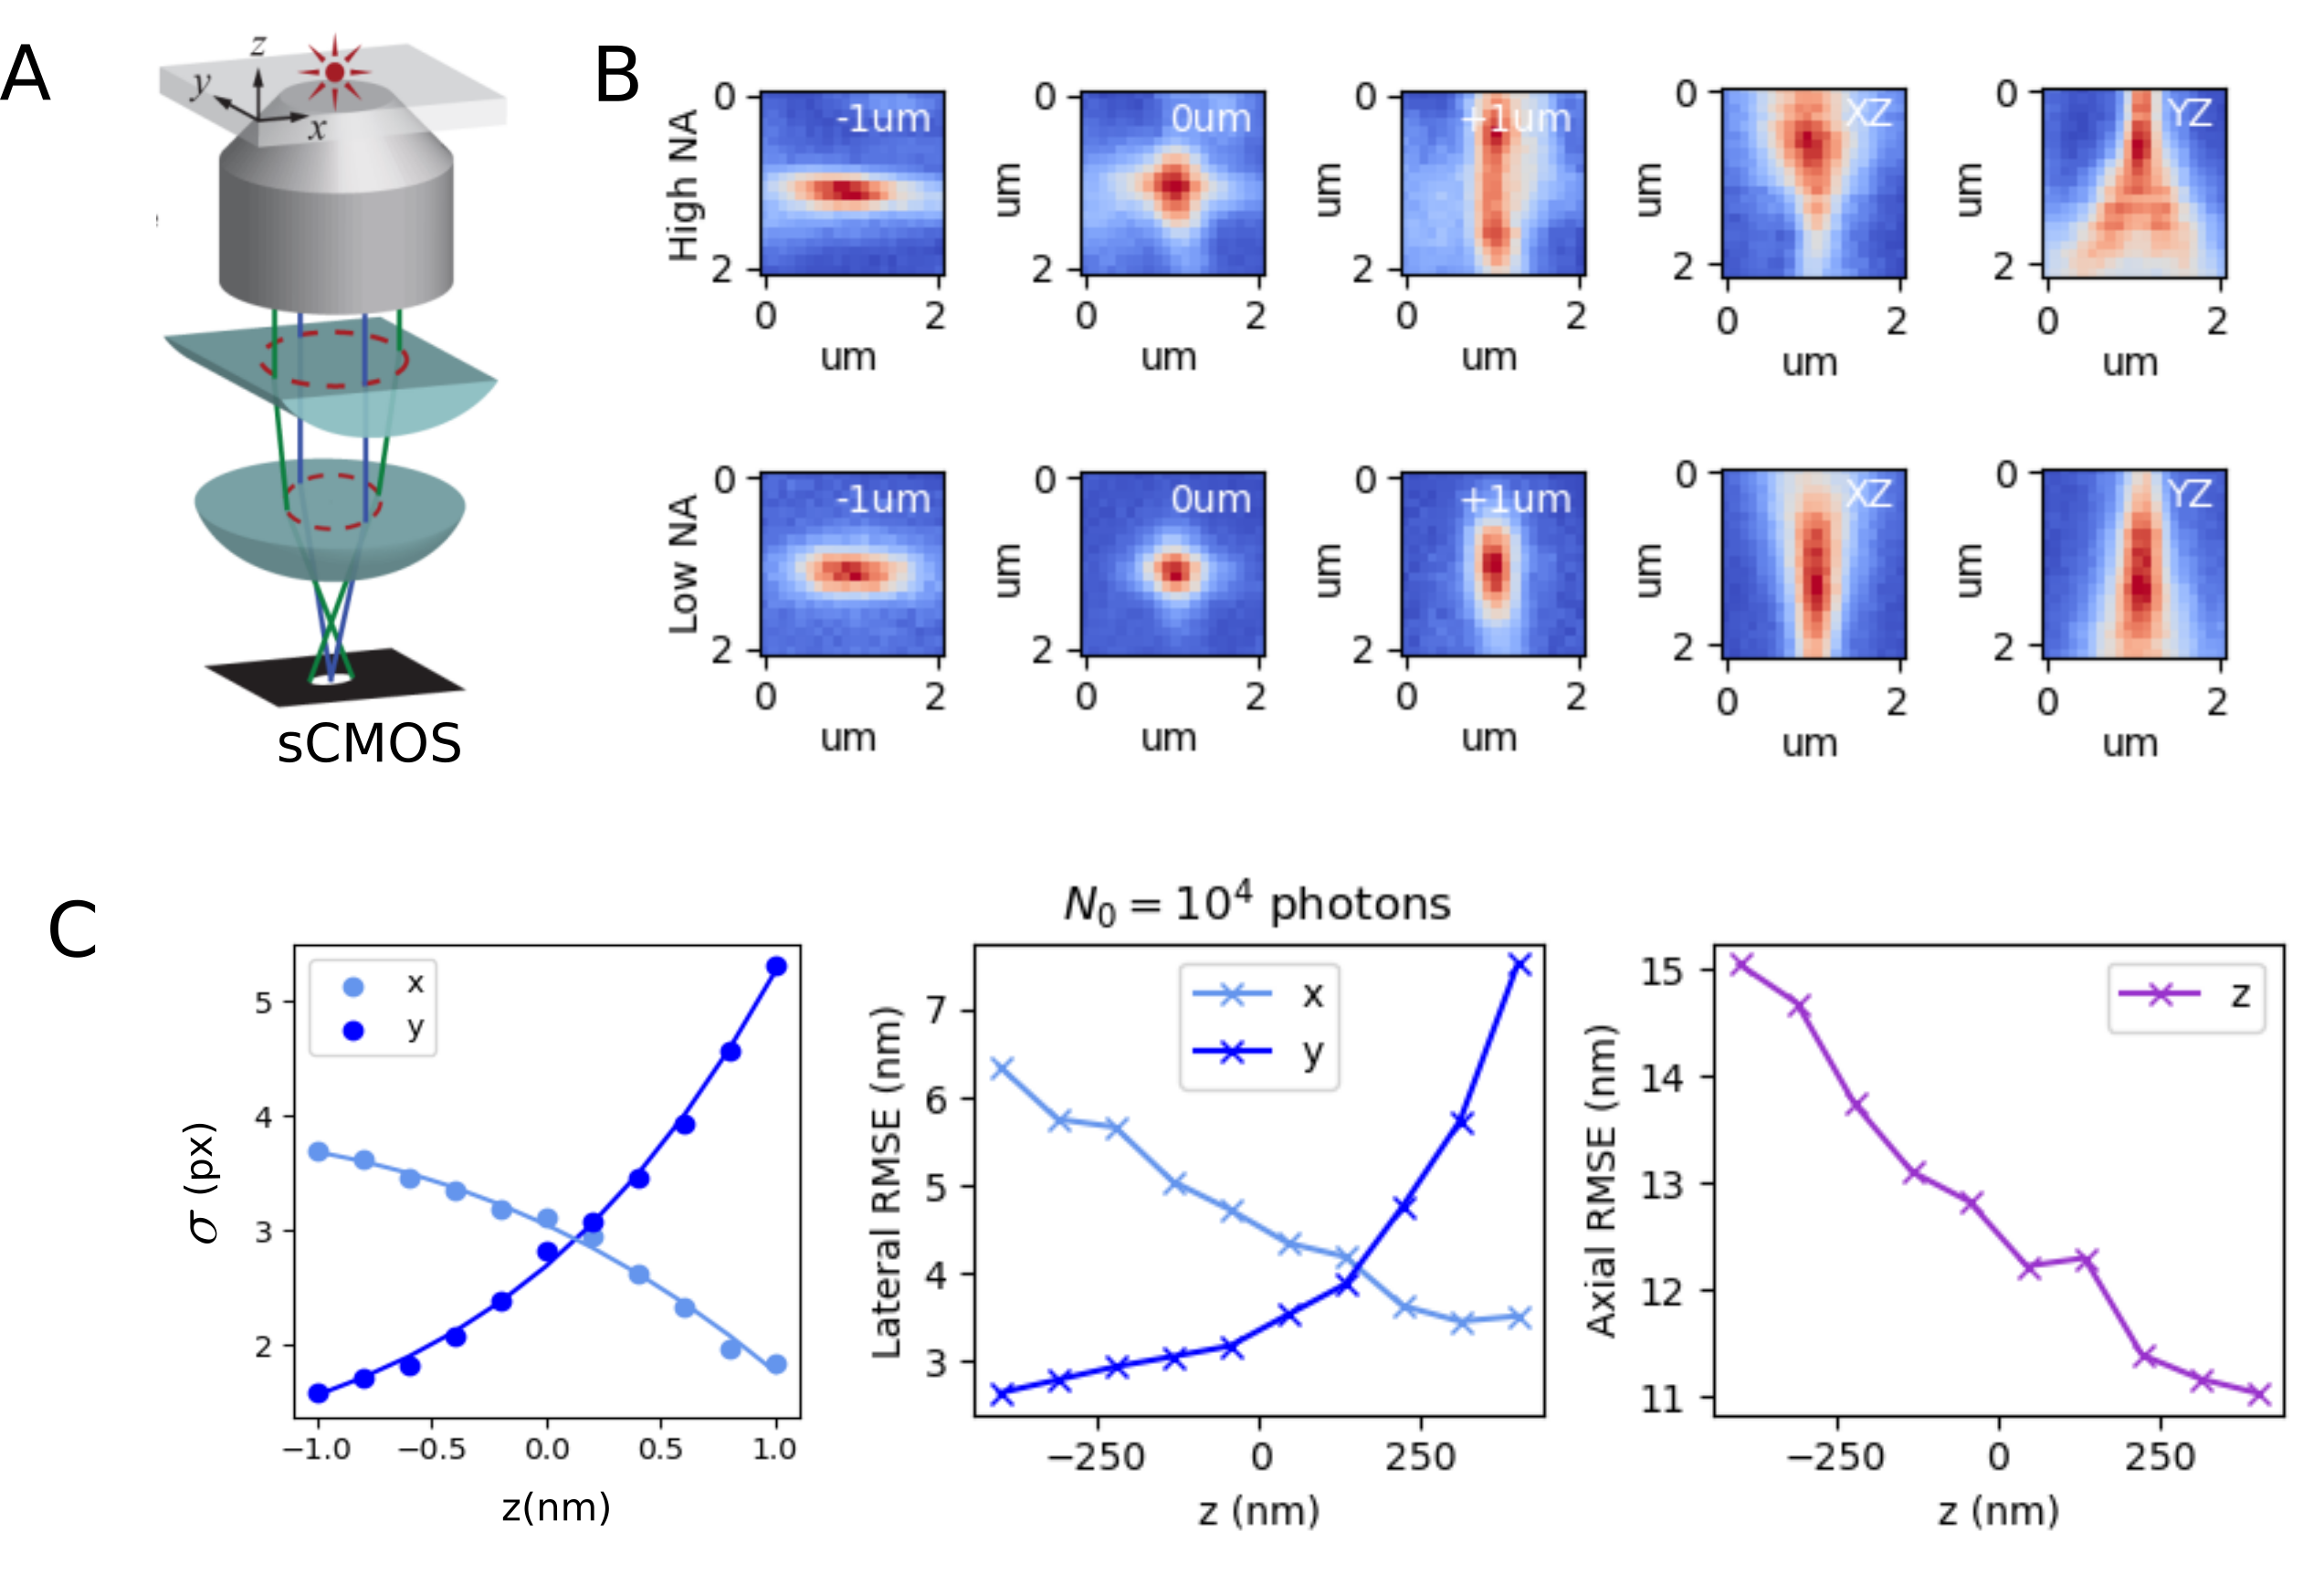
\includegraphics[width=14cm]{Astigmatism.png}
\end{center}
\caption{Axial precision for three-dimensional localization at ideal SNR (A) Simplified lens relay for astigmatic imaging of a fluorescent emitter using a weak cylindrical lens ($f$=10m). (B) Lateral and axial point spread function of a single quantum dot on a 1.5 glass coverslip for high ($\sim$1.25) and low ($\sim$0.8) numerical aperture (NA). (C) Polynomial fit of the standard deviation of the lateral point spread function along orthogonal axes (left) Root mean squared error (RMSE) of lateral coordinates as a function of the axial coordinate, using simulated images fit with MLE (middle). RMSE of the axial coordinate, using simulated images fit with MLE (right). Error samples = $10^{3}$}
\end{figure}

\subsection{Visualizing nucleosome cluster dynamics in BRD4 condensates at super-resolution}

Phase separation of chromatin and chromatin-associated proteins can be achieved in minutes, making it a suitable system for application for live cell super-resolution of chromatin structural dynamics (Itoh 2021). Previous approaches to studying the dynamics of chromatin nanodomains only provide ensemble snapshots of chromatin structure due to slow acquisition times (Nozaki 2017). Ensemble snapshots are a convenient choice in this context, yet biological systems are highly heterogeneous, and this precludes the observation of chromatin structure and residency of various chromatin modifiers. HaloTag fusion protein and its associated JF549-HaloTag and JF646-HaloTag ligands have surfaced as indispensable tools (Grimm 2015). H2B is a suitable choice, since it is one of the histones with fewer tail modifications and functional variants with known function (Kamakaka 2005).

\begin{figure}
\begin{center}
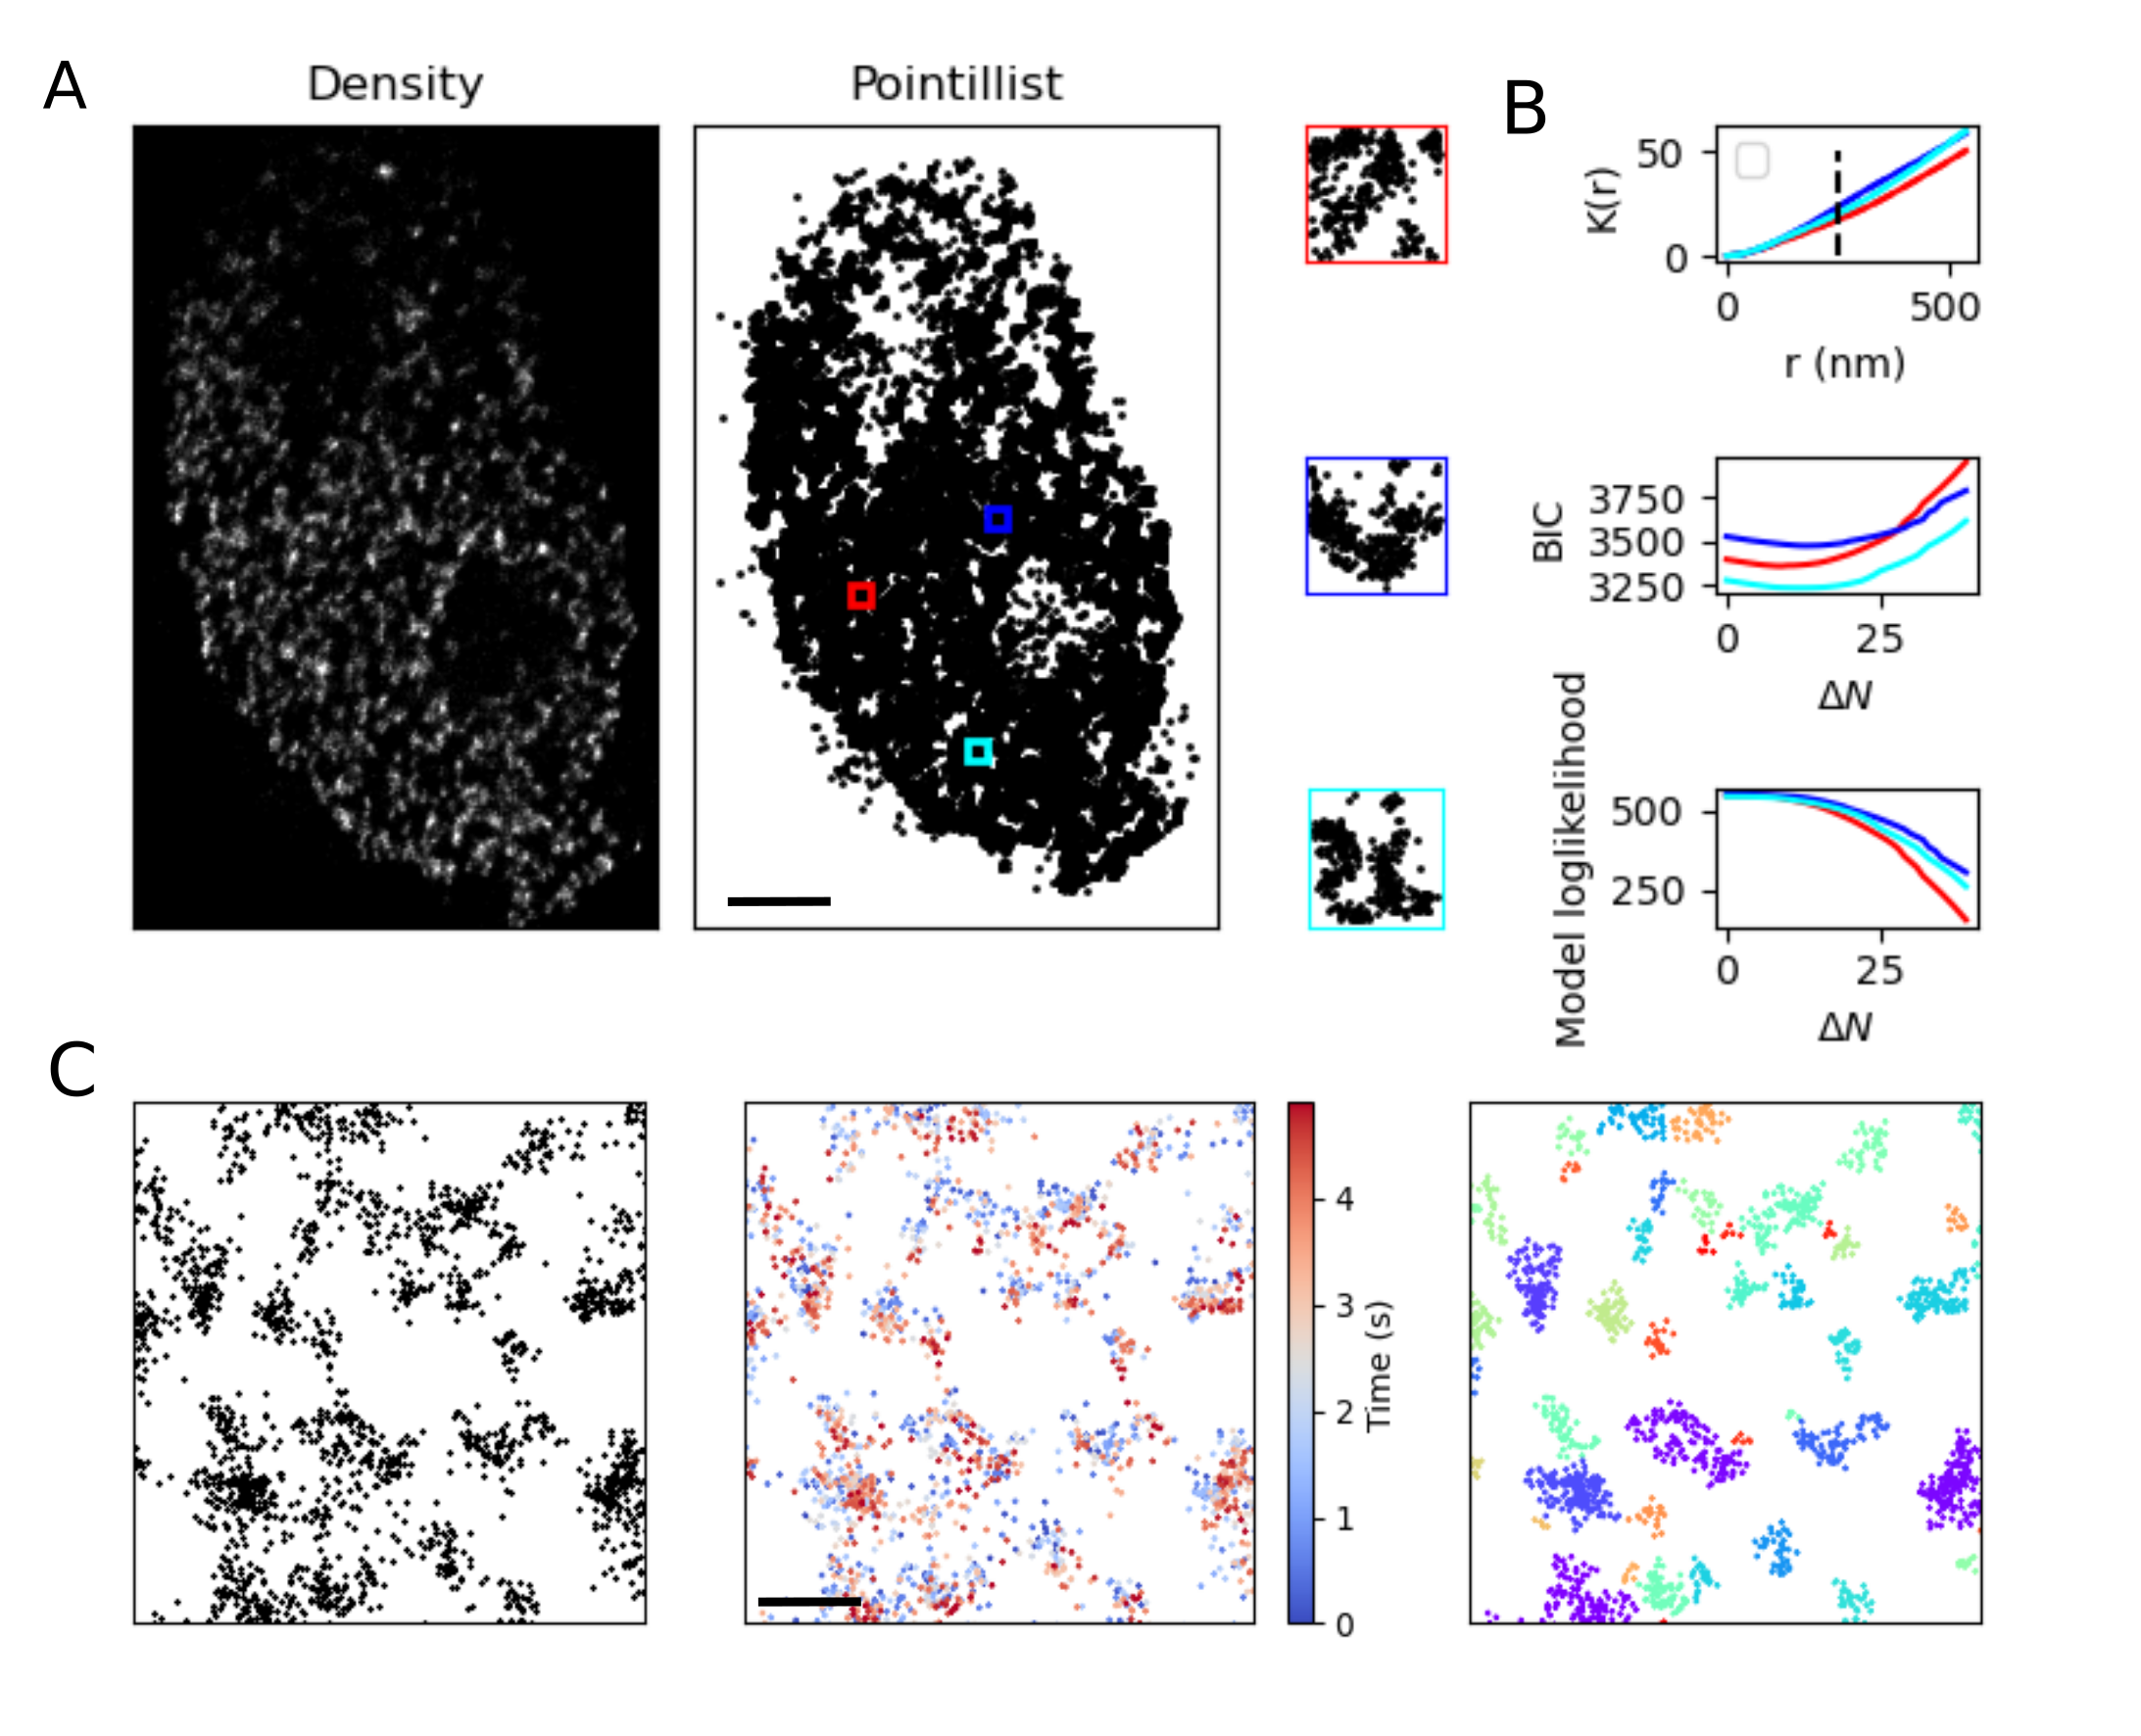
\includegraphics[width=16cm]{ClusterFull.png}
\end{center}
\caption{Super-resolution reconstruction of nucleosome organization in a living Hela cell nucleus. (A) Density representation of nucleosome organization using 30nm x 30nm bins and a pointillist representation of nucleosome organization (B) Ripley's K function, Bayesian information criterion (BIC), and log likelihood for a Gaussian mixture model of pointillist localization data of three randomly selected regions of interest (C) Localization accumulation over five seconds of imaging time (500 frames) and clustering with DBSCAN for a randomly selected region of interest}
\end{figure}

Here, we use the HaloTag system, a modified haloalkane dehalogenase designed to covalently bind to synthetic ligands  (Los 2008). The HaloTag protein is fused to H2B, either through transfection and clonal selection, or by transient transfection. The HaloTag is bound by a rhodomine-derived fluorescent ligands, JF549 or JF646, in order to (Grimm 2015). For super-resolution or three-dimensional single molecule tracking, we use oblique illumination microscopy to illuminate a thin area within a single nucleus (Tokunga 2008; Nozaki 2017). In dSTORM microscopy, the dark state lifetime of a fluorescent molecule can be tuned with illumination intensity (van de Linde 2011). This permits simultaneous single molecule tracking of H2B-JF549 and H2B-JF646 over several minutes. 

\subsection{Inhibition of a BRD4-controlled gene with JQ1}

\begin{figure}
\begin{center}
\includegraphics[width=16cm]{GBP5.png}
\end{center}
\caption{\textbf{Validation of induction of target gene GBP5 and JQ1 inhibition}. (A) Putative GBP5 transcription sites at the specified time points following IFN-$\gamma$ exposure. (B,C) High resolution zoom of GBP5 in-situ hybridization 8 hours folowing IFN-$\gamma$ exposure (D) Induction of GBP5 expression in Hela cells following IFN-$\gamma$ exposure, measured with RT-qPCR (E) Knockdown of GBP5 expression 8 hours folowing IFN-$\gamma$ exposure with 1uM JQ1 treatment (** P < 0.01) (F) Western blot of GBP5 protein expression following IFN-$\gamma$ exposure}
\end{figure}

\clearpage
\section{Future Aims}

\subsection{Specific Aim 1: Measure nucleosome cluster dynamics in living cells}

\subsubsection{Rationale and hypothesis}

So far, super-resolved nucleosome clustering has been predominantly studied in fixed cells (Nozaki 2017; Itoh 2021). Live cell studies are limited by the low time resolution of SMLM and have so far relied on reconstruction of nucleosome reorganization by transforming widefield images with convolutional neural networks. Using this techinque, it has been reported that nucleosome clusters reorganize on millisecond to second time scales (Barth 2020).  Therefore, we seek to apply our method to validate this result with fast two-color dSTORM microscopy on second time scales. 

\subsubsection{Experimental Approach}

To perform this experiment, we have optimized simutaneous two-color labeling of H2B-HaloTag with JF549 and JF646. We maintain sparse labeling of H2B with JF549 using 10pM concentration and a short incubation time of 1 hour. The purpose of using JF549 is two fold: (i) single molecule tracking can be performed on sparsely labeled samples with lower laser power than used in dSTORM (ii) Low laser power allows us to use this channel for autofocusing of the sample and performing cyclical imaging of the same living cell, with lesser photodamage. Moreover, we maintain dense labeling of H2B-HaloTag with JF646 for super-resolution imaging of nucleosome clusters. Experiments will be carried out on a live cell microscope based on an Olympus IX83.


\subsection{Specific Aim 2: Compare the effects of JQ1 and 1,6 Hexanediol exposure on BRD4 residency in Hela nuclei}


\subsubsection{Rationale and hypothesis}

Our previous results have validated the efficacy of JQ1 in inhibiting the expression of BRD4-controlled gene GBP5. This result is consistent with previous colocalization studies of the GBP locus with MED1 and BRD4 and identification of the GBP super enhancer (Lin 2022). JQ1 is a cell permeable small molecule that binds competitively to the acetyl-lysine binding cavity of BRD4, displacing BRD4 from chromatin (Fillappakopoulos 2010). BRD4 is known to play a role in nucleosome eviction as well as phase separation in nuclear bodies; however, it remains unclear the primary effects of BRD4 on nucleosome organization. JQ1 does indeed inhibit an array of genes, including GBP5 (Hogg 2017), but has had an insigificant effect on overall BRD4 residency in C33A nuclei (Han 2020). Therefore, it appears that the epigenetic role of BRD4 is more nuanced. For example, super-enhancers are far more sensitive to drugs blocking the binding of BRD4 to acetylated chromatin (Chapuy 2013; Loven 2013; Hnisz 2017). We hypothesize that large BRD4 aggregates are more susceptible to JQ1, while small aggregates can be dissolved with phase separation inhibitors, but not BET inhibitors alone.

1,6-hexanediol (1,6-HD), an aliphatic alcohol, can inhibit weak hydrophobic protein-protein interactions required for the droplet formation (droplet melting activity) and is widely used to elucidate the formation process of nuclear bodies. 1,6 Hexanediol is widely used as a control to dissolve phase separated assemblies in cells (Duster 2021). Exposure can rapidly induce broad reorganization of chromatin, providing a useful control for directly observing nucleosome cluster dynamics in mammalian cells. Nevertheless, changes in chromatin architecture following dissolution of epigentic proteins such as BRD4 (Sabari 2018) can be difficult to decouple from induced changes in chromatin structure itself. Previous studies have demonstrated in fixed cells that nucleosome clusters are rapidly immobilized and condensed after exposure to 1,6 Hexanediol (Itoh 2021). However, nucleosome organization is highly irregular and heterogeneous (Ricci 2015), making ensemble statistics inappropriate for making strong conclusions in fast perturbation experiments. 

\subsubsection{Experimental Approach}

JQ1 is a relatively slow acting small molecule drug. Therefore, we propose fixed cell experiments to validate its effect on BRD4 residency in the nucleus 2h, 4h, and 8h after exposure to 20uM JQ1. In fixed cell ensembles, we will measure size distributions of BRD4 clusters in control versus JQ1 treated cells. Later, we will transiently transfect BRD4-GFP fusion protein into Hela cells followed by three-color live cell imaging of BRD4, H2B-JF549, and H2B-JF646 following initial exposure to 1-5 percent 1,6 Hexanediol. Cells will be exposed to Hexanediol on the microscope stage, followed by cyclic super-resolution imaging. This phase wil be used to determine the effects of Hexanediol exposure on BRD4 residency in the nucleus and differential effects of Hexanediol on BRD4-positive and BRD4-negative chromatin nanodomains. 

\section{Materials and Methods}

\subsection{Cell lines, cell culture conditions, and transfection}

Hela cells were cultured in DMEM supplemented with 10  percent  fetal bovine serum (Gibco) at 37C, 5  percent  CO2 in a humidified incubator. Cultures were tested routinely for mycoplasma contamination; all tests were negative. For super-resolution experiments, cells were seeded in a 35mm FluoroDish (WPI), and transiently transfected with pBREBACK-H2BHalo plasmid (Addgene plasmid 91564) using Lipofectamine 3000 (ThermoFisher). 

\subsection{Interferon priming and other chemical treatments}

For immune activation, cells were incubated with 50ng/ml Interferon-gamma (Gibco), diluted in fresh DMEM. BRD4 inhibition experiments were carried out using 1uM JQ1 (Chemie Tek).  

\subsection{RNA fluorescence in-situ hybridization}

Cells were seeded in 8-well chamber slides with 1.5 glass coverslip bottom (Ibidi). GBP5 expression was induced with 50ng/ml Interferon-gamma, followed by fixation. Stellaris RNA FISH Wash Buffer A (Biosearch Technologies, Inc., SMF-WA1-60), 10  percent  Deionized Formamide (EMD Millipore, S4117) in RNase-free water (Life Technologies, AM9932) for 5 min at RT. Cells were hybridized with 90  percent  Stellaris RNA FISH Hybridization Buffer (Biosearch Technologies, SMF-HB1-10), 10  percent  Deionized Formamide, 12.5 µM Stellaris RNA FISH probes designed to hybridize introns of the . Hybridization was performed in a humidified chamber at 37C. Cells were then washed with Wash Buffer A for 30 min at 37°C and nuclei were stained with 15ng/ml DAPI in Wash Buffer A for 5 min at RT. After one 5-min was with Stellaris RNA FISH Wash Buffer B (Biosearch Technologies, SMF-WB1-20) at RT. Images were acquired as 10x10 grids on an ASI RAMM widefield microscope with 60X 1.4NA Nikon oil-immersion objective using Micromanager acquisition software and a Hammamatsu ORCA-Flash4.0v3 camera.  

RNA FISH probes were designed and generated by Biosearch Technologies Stellaris RNA FISH to target exons of GBP5. See Table 1 for the sequences of RNA-FISH probes.  

\subsection{Immunofluorescence}

Cells grown in chamber slides or 35mm dishes were permeabilized with 0.3  percent  (v/v) Triton-X100 (Sigma-Aldrich) in PBS and blocked for 1h in 5  percent  (w/v) nonfat dry milk at 4C. Cells were incubated overnight at 4C using primary antibodies anti-MED1 (Cell Signaling, clone E2A7X; 1:1000), and anti-BRD4 (Cell Signaling, clone E2A7X; 1:1000). Secondary antibodies for BRD4 (Cell Signaling Anti-Rabbit igG-Alexa488, 1:1000) and MED1 (Cell Signaling Anti-Rabbit igG-Alexa488, 1:1000) were used. 

\subsection{Quantitative reverse transcription polymerase chain reaction}

GBP5 induction was validated with RT-qPCR, using the TaqMan gene expression assay. Relative mRNA levels were computed using the delta-delta Ct method (Schmittgen 2008). 

\subsection{Immunoblotting}

Cells were washed and lysis buffer added (RIPA buffer: PMSF: protease inhibitor cocktail: orthovanadate=100:1:1:1). Cells were then scraped and sonicated for 15 seconds using an ultrasonic homogenizer. Lysate was centrifuged at high speed (13200r/min) for 10-15 minutes at 4C to pellet the cellular debris. Total protein concentration was determined by a BCA Protein Assay Kit (Pierce). For electrophoresis, protein samples were prepared according to a protein-loading ratio of 3:1. Sample was mixed and heated at 95℃ for 5 min, followed by vortex and centrifuge. After running the gel, it was removed from the cassette and assembled inside the Trans-Blot Turbo Transfer System cassette. Transfer was run at 2.5A for 7min. Sample was then blocked using 5  percent  skim milk blocking solution prepared with PBST. Primary GBP5 antibody was diluted with PBST (1:1000) and incubated at 4C overnight. The secondary antibody was diluted with PBST (1:2000) and placed on a rocker and incubate at RT for 45min. Western blots on PVDF membranes were scanned using the Odyssey fluorescence scanning system software. 

\subsection{Super-resolution imaging of nucleosome nanodomains}

After transient transfection, H2B-Halotag Hela cells were incubated with 50pM JF646 HaloTag ligand overnight, washed three times with PBS, and fixed with formaldehyde. Fixed Hela cells were imaged in a dSTORM photoswitching buffer containing 100mM MEA, 50 ug/ml Glucose Oxidase, and 3.4 mg/ml Catalase (Sigma). Buffer pH was adjusted to ~8 using HCl. Movies were collected using a custom Olympus IX83 microscope body equipped with an Olympus 60X 1.25NA oil-immersion objective. Images were projected onto an ORCA-Fusion sCMOS camera (Hamamatsu). The microscope was controlled using Micromanager software. HaloTag-JF646 molecules were illuminated with a 640nm laser held at 20mW (measured at the back focal plane of the objective).  5000 frames were captured at 100fps. Three-dimensional astigmatism time-series were captured by placing a cylindrical lens with 10m focal length (Optical Technologies) in the emission path of the microscope.  

Registration of movies was perform with StackReg rigid body registration. 

\subsection{Maximum likelihood estimation of molecular coordinates}

For each pixel, the number of photoelectrons $S_{k}$ is  multiplied by a gain factor $g_{k} \;[\mathrm{ADU}/e^{-}]$, which generally must be measured during calibration. The readout noise per pixel $\xi_{k}$ is Gaussian with some pixel-specific offset $o_{k}$ (Figure 2a) and variance $\sigma_{k}^{2}$ (Figure 2b). Ultimately, we have a Poisson component of the noise, which scales with the signal level and a Gaussian component, which does not. Therefore, in a single exposure, we measure: 

\begin{equation}
\vec{H} = \vec{S} + \vec{\xi}
\end{equation}

What we are after is the joint distribution $P(\vec{H})$. Fundamental probability theory states that the distribution of $H_{k}$ is the convolution of the distributions of $S_{k}$ and $\xi_{k}$,

\begin{align}
P(H_{k}|\theta) &= P(S_{k})\circledast P(\xi_{k})\\
&= A\sum_{q=0}^{\infty} \frac{1}{q!}e^{-\mu_{k}}\mu_{k}^{q}\frac{1}{\sqrt{2\pi}\sigma_{k}}e^{-\frac{(H_{k}-g_{k}q-o_{k})}{2\sigma_{k}^{2}}}
\end{align}

where $P(\xi_{k}) = \mathcal{N}(o_{k},\sigma_{k}^{2})$ and $P(S_{k}) = \mathrm{Poisson}(g_{k}\mu_{k})$,  $A$ is some normalization constant and $\circledast$ represents convolution. In practice, this expression is difficult to work with, so we look for an approximation. We will use the Poisson-Normal approximation to simplify Eq (4)

\begin{equation*}
\xi_{k} - o_{k} + \sigma_{k}^{2} \sim \mathcal{N}(\sigma_{k}^{2},\sigma_{k}^{2}) \approx \mathrm{Poisson}(\sigma_{k}^{2})
\end{equation*}

Since $H_{k} = S_{k} + \xi_{k}$, we transform $H_{k}' = H_{k} - o_{k} + \sigma_{k}^{2}$, which is distributed according to 

\begin{equation*}
H_{k}' \sim \mathrm{Poisson}(\mu_{k}')
\end{equation*}

where $\mu_{k}' = g_{k}\mu_{k} + \sigma_{k}^{2}$. This result can be seen from the fact the the convolution of two Poisson distributions is also Poisson. The quality of this approximation will degrade with decreasing signal level, since the Poisson distribution does not retain its Gaussian shape at low expected counts. Nevertheless, the quality of the approximation appears to increase exponentially with the expected count, as measured by the Komogonov distance between the convolution distribution (4) and its Poisson approximation (Figure 2c).

Localization microscopy supposes that molecules really do have an exact location in space. In pratice, this is only an approximation since molecules can diffuse at physiological temperatures, and our exposure time would need to tend to zero for this to be exactly true. If we suppose that we can collect a sufficient amount of photons in a short enough time, such that a definite position exists, the following optimization problem is defined

\begin{equation*}
\theta_{\mathrm{MLE}} = \underset{\theta}{\mathrm{argmax}}\prod_{k}P(H_{k}|\theta)= \underset{\theta}{\mathrm{argmin}}-\sum_{k}\log P(H_{k}|\theta)
\end{equation*}


where $\theta_{\mathrm{MLE}}$ represents the maximum likelihood coordinates of a fluorescent molecule. Maximum likelihood estimation (MLE) is a natural choice, since optimization of coordinates under a Poisson likelihood is tractable. Under the Poisson approximation, the model negative log-likelihood is

\begin{align}
\ell(\vec{H}|\theta) &= -\log \prod_{k} \frac{e^{-\left(\mu_{k}'\right)}\left(\mu_{k}'\right)^{n_{k}}}{n_{k}!}\\
&= \sum_{k}  \log n_{k}! + \mu_{k}' - n_{k}\log\left(\mu_{k}'\right)
\end{align}

First order derivatives of the above sum can often be computed analytically, depending on the spatial function $\mu$. The Poisson approximation is also convenient for computing the Fisher information matrix for $\theta_{\mathrm{MLE}}$ and thus the Cramer-Rao lower bound, which bounds the variance of a statistical estimator of $\theta_{\mathrm{MLE}}$, from below (Chao 2016).

\subsection{Dense localization with convolutional neural networks}

\subsection{Uncertainty quantification with Markov Chain Monte Carlo}

\subsection{Gaussian mixture model for correcting localization artifacts}

\section{Supplemental Information}

\begin{figure}
\begin{center}
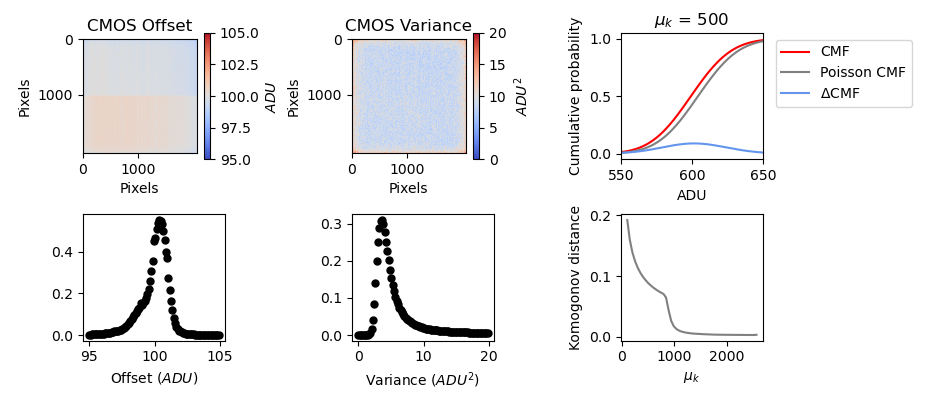
\includegraphics[width=16cm]{Noise.png}
\end{center}
\caption{Noise characterization of Hamamatsu ORCA-Flash 4 CMOS sensor. (A) Offset for zero incident photons (B) Variance for zero incident photons (C) Cumulative mass function for the convolution distribution and its Poisson approximation for rate parameter $\mu_{k} = 500$ counts (D) Komogonov distance measured as a function of rate parameter $\mu_{k}$}
\end{figure}

\begin{figure}
\begin{center}
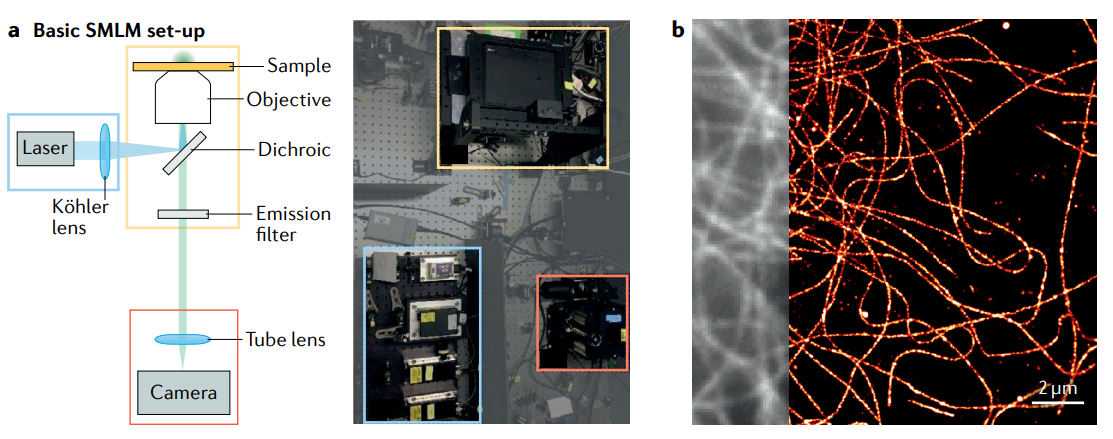
\includegraphics[width=14cm]{Setup.png}
\end{center}


\caption{Fluorescence microscopy setup for super-resolution and three-dimensional single molecule tracking. (A) Laser engine and two-path optical relay for selectable EPI with beam expansion (widefield) or HILO illumination based around the ASI RAMM modular system (B) Custom Olympus IX83 build with removable cylindrical lens for three-dimensional single molecule tracking or HILO illumination}
\end{figure}

\begin{figure}
\begin{center}
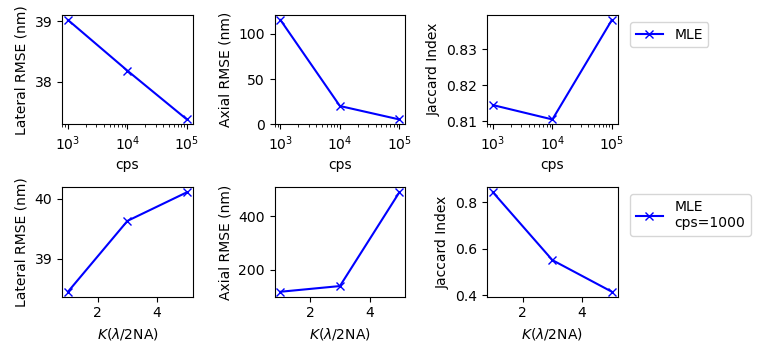
\includegraphics[width=16cm]{PSF3D.png}
\end{center}
\caption{Dependence of axial and lateral precision on SNR and molecular density. (upper row) Lateral and axial root mean squared errors (RMSE) at varying signal levels (lower row) Lateral and axial RMSE for varying molecule counts within a diffraction limit radius for $10^{3}$ photon counts. Error samples = $10^{3}$}
\end{figure}




\subsection{Integrated isotropic and anisotropic Gaussian point spread functions}


Due to diffraction, any point emitter, such as a single fluorescent molecule, will appear at the image plane as a diffraction limited spot. The diffraction limit $d = \lambda / 2\mathrm{NA}$ was first written down by Abbe, derived as the minimum separation between two objects such that they can still be optically resolved. For the sake of simplicity, it is common to describe the point spread function (PSF) as a two-dimensional isotropic Gaussian (Zhang 2007). This is an approximation to the more rigorous models given by Richards and Wolf (1959) or Gibson and Lanni (1989). 

\begin{equation*}
\mathrm{G}(x,y) = \frac{1}{2\pi\sigma^{2}}e^{-\frac{(x-x_{0})^{2}+(y-y_{0})^{2}}{2\sigma^{2}}}
\end{equation*}

The chracteristic width $\sigma$ of the PSF typically depends on the numerical aperture of the objective lens and The image of a fluorescent molecule captured by the objective lens, can be thought of as two-dimensional histogram of photon arrivals and a discretized form of the classical intensity profile $\mathrm{G}(x,y)$. The value at a pixel approaches an integral of this density over the pixel:

\begin{equation}
\mu_{k} = i_{0}\lambda_{k} = i_{0}\int_{\mathrm{pixel}} G(x,y)dxdy
\end{equation}


Let $(x_{k},y_{k})$ be the center of pixel $k$. If a fluorescent molecule is located at $(x_{0},y_{0})$, the probability of a photon arriving at pixel $k$ per unit time reads

\begin{align*}
\lambda_{k} = \int_{x_{k}-\frac{1}{2}}^{x_{k}+\frac{1}{2}}G(x-x_{0})dx \int_{y_{k}-\frac{1}{2}}^{y_{k}+\frac{1}{2}} G(y-y_{0})dy
\end{align*}

where $i_{0} = g_{k}\eta N_{0}\Delta$. The parameter $\eta$ is the quantum efficiency and $\Delta$ is the exposure time. $N_{0}$ represents the number of photons emitted per unit time. We can then express the Gaussian integrals over a pixel by making use of the error function, giving a convenient expression for the fraction of photons which arrive at a pixel $k$

\begin{align*}
\lambda_{k} = \frac{1}{4}\left(\mathrm{erf}\left(\frac{x_{k}+\frac{1}{2}-x_{0}}{\sqrt{2}\sigma}\right) -\mathrm{erf}\left(\frac{x_{k}-\frac{1}{2}-x_{0}}{\sqrt{2}\sigma}\right)\right)\left(\mathrm{erf}\left(\frac{y_{k}+\frac{1}{2}-y_{0}}{\sqrt{2}\sigma}\right) -\mathrm{erf}\left(\frac{y_{k}-\frac{1}{2}-y_{0}}{\sqrt{2}\sigma}\right)\right)\\
\end{align*}

This result is the workhorse of much of the remaining analyses, allowing us to efficiently simulate images of single molecules and benchmark localization algorithms. It is also straightforward to generalize this result when $G$ is an anisotropic Gaussian, which is studied in (Figure 4).


\end{document}


